\documentclass[../masters.tex]{subfiles}

\begin{document}
\graphicspath{{./imgs/}{../imgs/}} %look for images

\section{Nonlinear Models}
In this section we still consider probabilistic graphical models of the form shown in Figure \ref{fig_linmod}. The variables retain their meaning as before but we generalise the model by dropping the linearity assumption. Unfortunately, this generalisation, although allowing us to expand our investigation to a much more expressive class of models, makes closed form solutions to the inference problem intractable in general.   
\begin{figure}[H] 
\centering
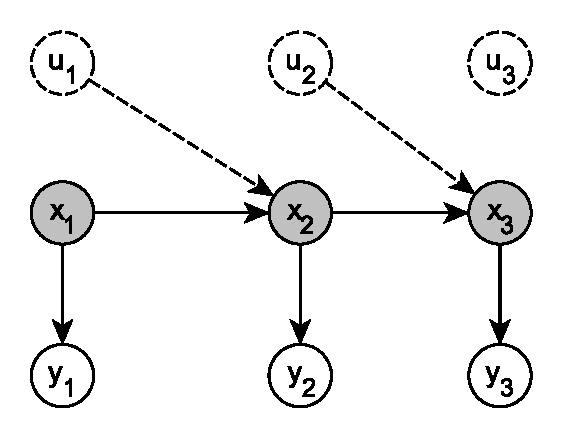
\includegraphics[scale=1.0]{linear_model.pdf}
\caption{Graphical model of this section}
\label{fig_linmod}
\end{figure}
We again assume that the transition and emission functions are time invariant. The state space model is now of the form (\ref{eq_statespace}).
\begin{equation}
\begin{aligned}
x_{t+1} &= f(x_t, u_t, w_{t+1}) \\
y_{t+1} &= g(x_{t+1}, v_{t+1})
\end{aligned}
\label{eq_statespace}
\end{equation}
Note that we make no assumption about the functional form of the noise terms $w_t,v_t$. In practice it is customary to assume that they have zero mean but otherwise are not restricted.

\subsection{Sequential Monte Carlo Methods}
Many approximate inference techniques exist in literature but we shall focus only on Sequential Monte Carlo (SMC) methods because it is simple to implement and generalises well (and easily) to more complex graphical models. 

SMC methods are a general class of Monte Carlo methods which sample sequentially from the growing target distribution $\pi_t(x_{1:t})$. By only requiring that $\gamma_t$ be known point-wise we have the framework of SMC methods as shown in (\ref{eq_SMC1}). Note that $Z_t$ is some normalisation constant \cite{pftut}.
\begin{equation}
\begin{aligned}
\pi_t(x_{1:t}) &= \frac{\gamma_t(x_{1:t})}{Z_t} \\
Z_t &= \int_{x_{1:t}} \gamma_t(x_{1:t})
\end{aligned}
\label{eq_SMC1}
\end{equation} 
In the context of filtering and prediction we will primarily only be interested in $\gamma_t(x_{1:t}) = p(x_{1:t},y_{1:t})$ and $Z_t = p(y_{1:t})$ so that $\pi_t(x_{1:t}) = p(x_{1:t}|y_{1:t})$. 

It is possible to approximate the distribution $\pi_t(x_{1:t})$ by drawing $N$ samples $X_{1:t}^i \backsim \pi_t(x_{1:t})$ and using the Monte Carlo method to find the approximation $\hat{\pi}_t(x_{1:t})$ as shown in (\ref{eq_SMC2}).
\begin{equation}
\hat{\pi}_t(x_{1:t}) = \frac{1}{N}\sum_{i=1}^N \delta(X^i_{1:t}, x_{1:t})
\label{eq_SMC2}
\end{equation}
We denote the Dirac Delta function of $x$ with mass located at $x_0$ by $\delta(x_0,x)$. It is easy to approximate the marginal $\pi_t(x_{t})$ as shown in (\ref{eq_SMC3}).
\begin{equation}
\hat{\pi}_t(x_{t}) = \frac{1}{N}\sum_{i=1}^N \delta(X^i_{t}, x_{t})
\label{eq_SMC3}
\end{equation}
It can be shown that the variance of the approximation error of $\pi_t$ decreases at rate $\mathcal{O}(\frac{1}{N})$. Unfortunately there are two significant drawbacks to the Monte Carlo approximation. The first is that often we cannot sample from $\pi_t(x_{1:t})$ directly and the second is that even if we could it is often computationally prohibitive. 

We use the Importance Sampling method to address the first problem. We do this by introducing an importance (sometimes called proposal) density $q_t(x_{1:t})$ such that $\pi_t(x_{1:t}) > 0 \implies q_t(x_{1:t}) > 0$. By substituting this into the SMC framework (\ref{eq_SMC1}) we have (\ref{eq_SMC4}).
\begin{equation}
\begin{aligned}
\pi_t(x_{1:t}) &= \frac{w_t(x_{1:t})q_t(x_{1:t})}{Z_t} \\
Z_t &= \int_{x_{1:t}} w_t(x_{1:t})q_t(x_{1:t})
\end{aligned}
\label{eq_SMC4}
\end{equation} 
Where we have defined the unnormalised weight function $w_t(x_{1:t}) = \frac{\gamma_t(x_{1:t})}{q_t(x_{1:t})}$. It is possible, for example, to set $q_t$ to a multivariate Gaussian which is easy to sample from. By drawing $N$ samples $X_{1:t}^i \backsim q_t(x_{1:t})$ and using (\ref{eq_SMC4}) we have (\ref{eq_SMC5}). 
\begin{equation}
\begin{aligned}
\hat{\pi}_t(x_{1:t}) &= \frac{1}{N}\sum_{i=1}^N W_t^i\delta(X^i_{1:t}, x_{1:t}) \\
\hat{Z}_t &= \frac{1}{N}\sum_{i=1}^N w_t(X^i_{1:t}) \\
W^i_t &= \frac{w_t(X^i_{1:t})}{\sum_{i=1}^N w_t(X^i_{1:t})}
\end{aligned}
\label{eq_SMC5}
\end{equation}
Now we will attempt to modify the Importance Sampling method to address the second problem of computational cost incurred by the sampling routine. 

We do this by selecting an importance/proposal distribution which factorises according to $q_t(x_{1:t}) = q_{t-1}(x_{1:t-1})q_t(x_{t}|x_{1:t-1}) = q_1(x_1) \Pi_{k=2}^t q_k(x_k|x_{1:k-1})$. In this way we only need to sample sequentially at each time step: at time $t=1$ we sample $X_1^i \backsim q_1(x_1)$, at time $t=2$ we sample $X_{2}^i \backsim q_2(x_2|x_1)$ and so we build up $X^i_{1:t} \backsim q_t(x_{1:t})$ factor by factor.

The weights can be written in the form (\ref{eq_SMC6}).
\begin{equation}
\begin{aligned}
w_t(x_{1:t}) &= \frac{\gamma_t(x_{1:t})}{q_t(x_{1:t})} \\
&= \frac{\gamma_{t-1}(x_{1:t-1})}{q_{t-1}(x_{1:t-1})}\frac{\gamma_t(x_{1:t})}{\gamma_{t-1}(x_{1:t-1})q_t(x_t|x_{1:t-1})} \\
&= w_{t-1}(x_{1:t-1})\alpha_t(x_{1:t-1}) \\
&= w_1(x_1)\Pi_{k=2}^t \alpha_k(x_{1:k})
\end{aligned}
\label{eq_SMC6}
\end{equation}
Thus, at any time $t$ we can obtain the estimates $\hat{\pi}_t(x_{1:t})$ and $Z_t$. The major limitation of this approach is that the variance of the resulting estimates typically increases exponentially with $t$ \cite{pftut}. 

We overcome this problem by resampling and thus introduce the Sequential Importance Resampling method. 

\bibliographystyle{plain}
\bibliography{research}

\end{document}